% -----------------------------------------------
% Template for SMC 2009
%     smc2009.sty -> style file
% Last modified by Fabien Gouyon (smc2009@inescporto.pt)
% Modified by Juan P. Bello (ismir2008-papers@ismir.net)
% By Rainer Typke (ismir07.rainer@safersignup.com)
% Based on the 2004 template by Eloi Batlle.
% -----------------------------------------------

\documentclass{article}
\usepackage{smc2009,amsmath}
% To use when using pdflatex
\usepackage{graphicx}
\usepackage{url}     
\usepackage{hyperref}   
      
\newenvironment{packed_item}{
\begin{itemize}
  \setlength{\itemsep}{1pt}
  \setlength{\parskip}{0pt}
  \setlength{\parsep}{0pt}
}{\end{itemize}}

\newenvironment{packed_enumerate}{
\begin{enumerate}
  \setlength{\itemsep}{1pt}
  \setlength{\parskip}{0pt}
  \setlength{\parsep}{0pt}
}{\end{enumerate}}
% To use when using latex, dvips and ps2pdf
% \usepackage[dvips]{graphicx}

% Title.
% ------
\title{Paper Template for SMC 2009}

% IMPORTANT NOTICE:
% Reviews are double-blind
% Authors will not be informed of who reviews their papers, and author names will be concealed from the reviewers 
% Please avoid evident self references in the text

% Authors' names must be omitted from title page (or listed as �name(s) omitted for submission�)


% Single address
% To use with only one author or several with the same address
% ---------------
%\oneauthor
%   {Author} {School \\ Email}

% Two addresses
 %--------------
\twoauthors
  {First author} {School \\ Email}
  {Second author} {Company \\ Email}

% Three addresses
% --------------
%\threeauthors
%  {First author} {School \\ Email}
%  {Second author} {Company \\ Email}
%  {Third author} {Company \\ Email}


\begin{document}
%
\maketitle
%

\permission

\begin{abstract} 
-flexible working environment for spatialization\\
-towards interoperability in sound spatialization management\\
The abstract should be placed at the top left column and should contain
about 150-200 words.
\end{abstract}

\section{Introduction - TL|NP}\label{sec:introduction}
%keywords: spatialization, adaptation, site-specific, Ambisonics, 
 
    
-Use cases (users : composers, installation artists, scientists...etc...)
   - OpenMusic off-line rendering
   - BEAST sound diffusion (the more speaker - the mre complicated to perform)
   - interactive sound installations
   - real-time control via sensors/gestural controller etc. by performer
   - tape-music (fixed media)
   - computer generated - real time spatialization (see <meta-description> layer)
   



Requirements for a spatialization framework at different levels in a compositional process.
Experimenting -- Composing -- Performance -- Documentation. The outlined requirements may differ according to artistic paradigms.  
    
%Experimental stage:\\
%\begin{packed_item}
% \item {Plug-In structure: exchangeable renderer and interface components} 
% \item {multichannel recording possibility for capturing of sketches/ideas}         
% \item {present management}
% \item {sound scene visualization - especially for off-line rendering of spatial processes}
%\end{packed_item} 

%Compositional stage:\\  
%\begin{packed_item}
%  \item {binaural rendering for headphone listening} 
%\end{packed_item} 
%Performance stage:\\
%\begin{packed_item} 
%	\item {customizable to accommodate for different technical conditions, e.g. rendering to different reproduction formats, compensation for non-ideal %loudspeaker configurations, routing signals to dedicated physical outputs}   
%    \item {testing technical setup, e.g. loudspeaker connections}
%    \item {customizable to accommodate for different acoustical conditions, e.g. adapting the virtual room description to the listening room} 
%\end{packed_item} 
%Documentation stage:\\  
%\begin{packed_item}
%\item {multichannel recording possibility}         
%\item {storing }       
%\end{packed_item}  
\begin{packed_item}
\item {separate render and control layer}
\item {Plug-In structure: exchangeable renderer and interface components}
\item {customizable to accommodate for different technical conditions, e.g. rendering to different reproduction formats, compensation for non-ideal loudspeaker configurations, routing signals to dedicated physical outputs}  
\item {customizable to accommodate for different acoustical conditions, e.g. adapting the virtual room description to the listening room} 
\item {allowing for external control e.g. through MIDI or OSC}
\item {present management}
\item {sound scene visualization}   
\item {binaural rendering for headphone listening}
\item {multichannel recording possibility} 
\item {testing technical setup, e.g. loudspeaker connections} 
\end{packed_item}	
   



%\quote{ What WE need, for our personal work, is a way to extend the capabilities of those tools in a completely flexible and configurable way - and that suggests plug-ins (though it will always be a potential problem overcoming inherent IO structures in the host applications).}

%\quote{working with non-standard loudspeakers: Meyer Sound Spherical Loudspeaker Array that is under research at CNMAT, or the Hemisphere Point-source Emanation Loudspeaker, for example.  I would like to experiment with these;}

%\quote{Tool building and music making happen together and depend upon each other.}

%\quote{Very frustrated with my current spatialization software and am desperately looking for something better!}

\section{Review}
This section gives an overview of  current paradigms and solutions for spatial sound synthesis. 


\subsection{digital audio workstations - DAW}   
- a lot of composer use DAW\\
- why?: composers are adapted to the concept and restrictions of DAWs\\
- - - good workflow and project management\\
- - - extendable through plugIns\\
- - - accomplished the goals for fixed media and tape-music and consumer media production\\


spatialization is mainly done in DAWs and leads to "panning" because the bus architectures and interfaces of the panning plugins suggests this.
    Limitations:
        a) mainly tied to consumer formats (stereo and ITU 5:1 surround)
        b) restricted to linear prerendering compositional processes
        c) complicated to maintain automation when changing rendering plugIn
        d) burden to connect interfaces (Lemur, Stantum, Wacom, Camera-tracking)
        
        <- BENJAMIN will write something about this (GUIs, multichannel audio routing in DAWs, adaptation to the listening room) -> 10/15 lines
        
\subsection{Media programming environments}
Beside the paradigm of the DAW, various media programming environment exist, such as SuperCollider, Pure Data, Chuck, Bidule, or Max/MSP which are capable for spatial sound synthesis in real-time. In order to support individual approaches and to meet the specific needs of computer music and mixed media art, these environments enable the user to combine music making with computer programming.  
However, in the name of complete flexibility, these environments lack in providing structured solutions for the specific challenges in spatial music, as outlined in section XYZ. Consequently, enumerable different self-contained libraries and spatialization toolboxes were created by artists and researcher, such as the Space Unit Generator \cite{SUG02}, IRCAM's Spatialisateur \cite{JotPhD} or Virtual Microphone Control \cite{CMJ08-VIMIC} to generate virtual sound sources and artificial spaces. Also frameworks primarily dedicated to sound diffusion practice, such as the BEASTmulch System\footnote{\url{http://www.beast.bham.ac.uk/research}}, or ICAST \cite{ICAST06} are available.   

\section{Strategies \& Methodologies in Spatial Sound Synthesis}  
- TROND, J45CH, NILS, PASCAL\\


a set of strategies to make working with spatialisation more flexible, modular, customizable and interoperable.\\
Eric Lyon: \cite{Lyon:2008spatial_orchestration}\\ 
   working symbolically?  - separating rendering and controlling algorithms\\
       are there other approaches? diffusion practice (e.g. acousmatic sound projection)? (specific editing to a fixed form)\\
   common interface
   modularity
   flexible (dynamic) number of channels 
   \url{http://en.wikipedia.org/wiki/OSI_model}


\subsection{hierarchical layers}
TROND, J45CH\\
\begin{packed_enumerate}   
\item[5.]{controlling the rendering (e.g. HoloEdit, ambicontrol, swarms, boids \cite{kimboyle:ssp}, trajectories...)     <indirect control description or meta-description> 
       Protocol: SpatDIF extended }
\item[4.]{position of sources and speakers at one moment in time as SpatDIF                          <direct control description>
       Protocol: SpatDIF core, SpatDIF extended if required by the encoder }
\item[3.]{encoded audio
       Protocols:
           Spatial infomation embedded in format: (e.g. B-format and Dirac, MPEG-surround ?)
           SpatDIF core and extended if required by the encoder (concerning info on target system) }
\item[2.]{decoded audio
       Protocols: E.g. CoreAudio, Jack }
\item[1.]{physical layer (computers, sound cards, speakers, etc.)}
\end{packed_enumerate}  



\section{Tools}
- structured according to layers

\subsection{ICST Ambisonics}
--> J45CH     
\cite{Schacher:2006ambi_max}, \cite{Neukom:2008ambipan}
\subsection{Jamoma}
(what is jamoma?, jamoma dsp, jamoma multicore, jamoma modular, dataspace lib) --> TIM    
 
\subsection{SpatDIF}
--> Nils 

\subsection{Holo-Edit}
--> Charles



\section{Style Stuff - delme}

\subsection{Title and Authors}

The title is 14pt Times, bold, caps, upper case, centered. Authors' names are centered. 
The lead author's name is to be listed first (left-most), and the co-authors' names after. If the addresses for all 
authors are the same, include the address only once, centered. If the authors have different addresses, 
put the addresses, evenly spaced, under each authors' name.

Reviews are double-blind. {\it \textbf{Author information should be removed from this page in initial submissions}}, 
and only added later by the authors when sending camera-ready versions.


\subsection{Figures, Tables and Captions}

All artwork must be centered, neat, clean, and legible. All lines should
be very dark for purposes of reproduction and art work should not be hand-drawn.
The proceedings is not in color, and therefore all figures must make
sense in black-and-white form.
Figure and table numbers and captions always appear below the figure. Leave 1
line space between the figure or table and the caption. Each figure or table
is numbered consecutively. Captions should be Times 10pt.
Place tables/figures in text as close to the reference as possible.
References to figures and tables should be capitalised, for example:
see Figure \ref{fig:example} and Table \ref{tab:example}.
Figures and tables may extend across both columns to a maximum
width of 7'' (17.78~cm).

\begin{table}
\begin{center}
\begin{tabular}{|l|l|}
\hline
String value & Numeric value \\
\hline
hello SMC  & 1073 \\
\hline
\end{tabular}
\end{center}
\caption{Table captions should be placed below the table}
\label{tab:example}
\end{table}

\begin{figure}
\centerline{\framebox{
% To use when using pdflatex
	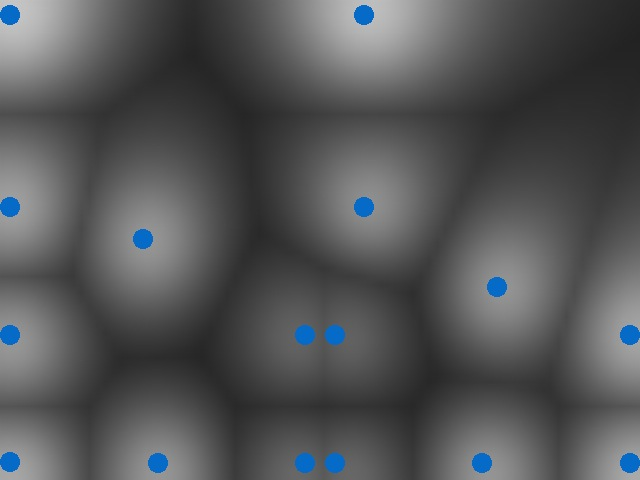
\includegraphics[width=\columnwidth]{../ICMC2009-dbap/all_r_6_b_0_2}}}
	% To use when using latex, dvips and ps2pdf
% 	
\includegraphics[width=\columnwidth]{figure.eps}}}
\caption{Figure captions should be placed below the figure}
\label{fig:example}
\end{figure}


\section{Discussion \& Outlook}

\section{Conclusion}
A conclusion is the place when you get tired of thinking. \\

\section{Acknowledgment}
\bibliographystyle{abbrv}  %\bibliographystyle{natbib}% ama, nar, alpha, plain, chicago,{plainnat}  abbrv, siam   
\small
\bibliography{smc09}
\end{document}   

%%%%%%%  Poubelle %%%%%%   
	
%\subsection{Frameworks for Spatialization}
%\textbf{Spatialisateur} (Spat) \cite{JotPhD}, in development at IRCAM and Espaces Nouveaux since 1991, is a library of spatialization algorithms for MaxMSP, including VBAP, first-order Ambisonics and stereo techniques (XY, MS, ORTF) for up to 8 loudspeakers. It can also reproduce 3D sound for headphones (binaural) or 2/4 loudspeakers (transaural). A room model is included to create artificial early reflections and reverb controlled by a perceptual-based user interface.\\
%\textbf{Ambisonics toolbox}  \cite{Schacher:2006ambi_max}

   
%
%\section{Taxonomy of Spatialization Modules in Jamoma}
%\subsection{Rendering Modules}
%\subsubsection{Ambisonics}
% \cite{Schacher:2006ambi_max}   
%Decoding/Adjusting/Encoding
%\subsubsection{VBAP}
%  \cite{Pulkki:2000vbap_max}
%\subsubsection{DBAP}
% \cite{dbapICMC09}
%\subsubsection{ViMiC}
%\cite{Peters:2008vimic} \cite{CMJ08-VIMIC}
%\subsubsection{binaural}
%?? Does anybody has a working module for this ?
%\subsection{Control Modules}
%\subsubsection{HoloEdit Modules}
%-  holo.transport\\
%-  holo.reccontrol\\ 
%paper ?
%\subsubsection{Geotransforms}
%- scene3D
%\subsection{mappings}
%- boids3D 
%\subsection{Effect Modules}
%\subsubsection{Doppler}
%\subsubsection{Airfilter}
%\subsubsection{RollOff}
%\subsubsection{Reverb}  
%\subsection{Utilities}
%\subsubsection{loudspeaker setup and correction}
%-sur.speaker.setup             \\
%-sur.distamp$\sim$   \hspace{2cm}SPL compensation\\
%-sur.speaker.delay$\sim$ \hspace{2cm}delay compensation        \\
%\subsubsection{multichannel tools}
%- meters\\
%- aux \\



